\subsection{Study of the Relativistic NN Bound System}

One of the important issues in studying of nuclear structure  at short distances is the 
relativistic description of the bound system.  This is an important issue also in 
understanding the QCD medium effect with recent studies indicating that  parton distribution 
modifications  in nuclei are proportional to the high momentum component of nuclear wave function.

The deuteron is the simplest bound system and naturally any self-consistent attempt  to understand the 
relativistic effects in the bound nuclear systems  should start with the deuteron. 
The issue of the relativistic description of the deuteron has long history with extensive research that started in late 1970's~\cite{Gross:1982nz,Buck:1979ff,Frankfurt:1977vc,Frankfurt:1981mk}.

The experimental studies of the relativistic effects in the deuteron  up to now included the large $Q^2$ elastic 
$ed$ scattering~\cite{Alexa:1998fe}, however  
due to complexities  in the reaction mechanism~\cite{VanOrden:1995eg} the relativistic effects were 
difficult to isolate.

The inclusive D$(e,e')$X experiments from tensor-polarized deuteron at  $Q^2>1$~GeV$^2$ and $x>1$ region gives 
a new possibility to probe the relativistic structure of the deuteron.  In this case the use of the tensor polarized
deuteron allows us to prepare the nucleus in the most compact state in which, due to the absence of the 
pure S-wave$^2$ contribution, the system in average is sensitive to the higher moment of the nucleon in the deuteron.
At large $Q^2>1$ GeV$^2$ kinematics, the probed longitudinal momenta of the bound nucleon $p_z \approx m_N(1-x)$, 
or the light cone momentum fraction $\alpha \ge x$. Because of these kinematic conditions and the absence of the 
large S-wave$^2$ contribution, one expects a measurable relativistic effects already at $x\le 1.2$.  

The biggest advantage in this case is that, because relatively small values of the bound nucleon momenta involved ($\ge 200~\mathrm{MeV}/c$),
one expects less uncertainty due to the choice of the NN potential  and reaction dynamics.

The sensitivity to the relativistic effect is estimated using the theoretical calculations based on two 
very different approaches.   The first approach treats the  virtuality of the bound nucleon within a
description of the deuteron in the lab. frame  with treating the interacting nucleon as being 
virtual (virtual nucleon, or VN, approximation) 
by taking the residue over the energy of the spectator nucleon.
In this case, the deuteron wave function satisfies the covariant equation of two-nucleon bound system 
with spectator being on energy shell~\cite{Sargsian:2009hf,Gross:2010qm}.

 Another approach is based on the observation that high energy processes
evolve along the light-cone (LC).  Therefore, it is natural to describe the 
reaction within the light-cone non-covariant framework \cite{Frankfurt:1981mk}. 
Negative energy states do not enter in this case, though one has to take into 
account so called instantaneous interactions.
In the approximation when non-nucleonic degrees of freedom in the
deuteron wave function can be neglected, one can unambiguously relate
the light-cone wave functions to those calculated in the lab. frame
by introducing the LC $pn$ relative three momentum
$k=\sqrt{{m^2+p_t^2\over \alpha(2-\alpha)} - m^2}$.

In Fig.~\ref{fig:misak}, the prediction for VN~\cite{Sargsian:2009hf} and LC~\cite{Frankfurt:1993sp} approximations are given 
for the highest $Q^2$ kinematics proposed. As it was mentioned above the measurable 
differences is predicted already at $x\ge 1.2$ where one expect little uncertainty due 
to the choice of the wave function.  
 
 

\begin{figure}
\begin{center}
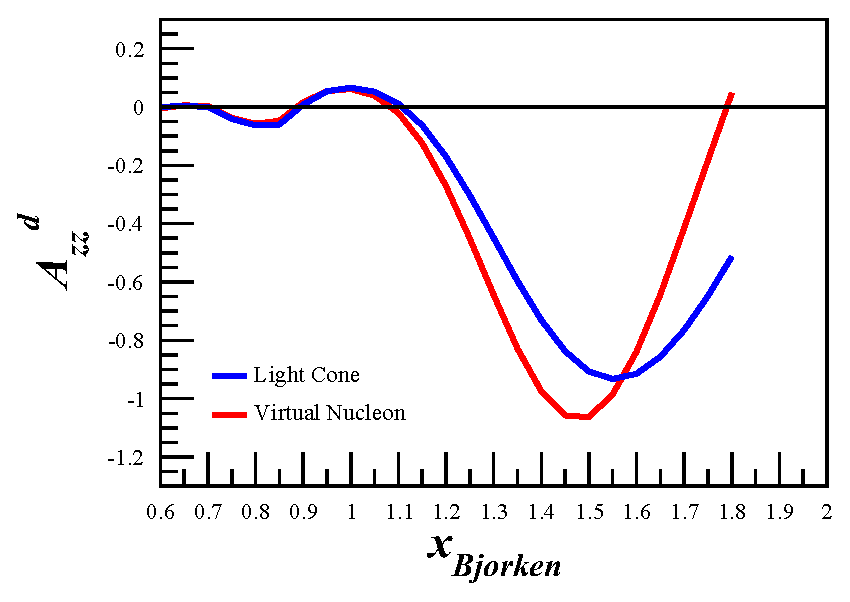
\includegraphics[width=0.50\textwidth]{figs/misak_vn_lc.eps}
\caption{\label{fig:misak} The $A_{zz}$ observable calculated at $Q^2=1.5~(\mathrm{GeV}/c)^2$ using the light-cone and virtual nucleon models. Calculations provided by M. Sargsian.}
\end{center}
\end{figure}

